%!TEX root = twig-language.tex

\section{Code generation}
\label{sec:code-gen}

One of our goals for Twig was that it be able to generate code in many different target languages. To that end, Twig's semantics rely on an abstract, language-independent model for code generation, with a small number of basic operations. To incorporate a new target language, it suffices to implement only these operations. There is no need to modify the core Twig interpreter, which assumes nothing beyond the abstract model.

Our simplified code generation model is used in formulating Twig's core semantics, described in Section~\ref{sec:semantics}. It is also helpful in clarifying the precise operations which Twig supports, without getting bogged down in the (potentially rather complicated) details of outputting code for a particular target programming language.

In Section~\ref{sec:code-gen:abstract}, we describe the abstract code generation model, apart from any specific target programming language, including the formal semantics. Then, in Section~\ref{sec:code-gen:c} we show how we use the model to generate C code.

\subsection{Abstract Code Generation}
\label{sec:code-gen:abstract}

In Twig, a unit of code to be generated is called a \emph{block}. Intuitively, a block represents some code in the target language, which accepts inputs and produces outputs. We call the set blocks $M$, and we say that for all $x \in M$ we have the functions 

\begin{eqnarray*}
\mathtt{in} : M \to \mathbb{N}^0\\
\mathtt{out} : M \to \mathbb{N}^0
\end{eqnarray*}

That is, \texttt{in} and \texttt{out} will map a block to the  number of its inputs and outputs, respectively. Note that either or both may be zero for a given $x$.

\subsubsection{Sequential Composition}

The first of Twig's elementary block operations is called  \emph{sequential composition}, which we represent as addition ($+$). Intuitively, sequencing represents connecting two blocks  ``vertically,'' by feeding the outputs of the first block to the inputs of the second. Formally, we define the subset $x+y$ by

\[
\infer
  {x+y \in M}
  {x \in M \quad y \in M \quad \mathtt{out}(x) = \mathtt{in}(y)}
\]

\begin{eqnarray*}
\mathtt{in} (x+y) &\equiv& \mathtt{in}(x)\\
\mathtt{out}(x+y) &\equiv& \mathtt{out}(y)
\end{eqnarray*}

Note that the condition that the number of outputs on the left side be equal to the number of inputs on the right implies that $M$ is not closed under sequential composition. The result of sequencing blocks where the inputs and outputs are mismatched is undefined. We take care in the design of the rest of Twig's semantics to avoid this case.

\subsubsection{Parallel Composition}

The second elementary operator is called \emph{parallel composition}. We represent this operation with the multiplication operator ($\times$). Intuitively, parallel composition fuses two blocks ``horizontally,'' where each block executes independently of one another, but they appear as a single block with combined inputs and outputs. Formally, we define $\times$ as

\[
\infer
  {x \times y \in M}
  {x \in M \quad y \in M}
\]

and we define

\begin{eqnarray*}
\mathtt{in} (x \times y) &\equiv& \mathtt{in}(x)  + \mathtt{in}(y)\\ 
\mathtt{out}(x \times y) &\equiv& \mathtt{out}(x) + \mathtt{out}(y) \end{eqnarray*}

Note that $M$ is closed under parallel composition.

\subsubsection{Special Blocks}

In the abstract model, we single out a set of special elements in $M$ called \emph{permutation} elements. These elements are intended to represent the primitive operation of taking $m$ inputs and rearranging them into $n$ outputs, possibly in a different order, and possibly duplicating or dropping elements. The intended interpretation is that the actual values are unchanged by the operation. Formally, we name the block representing the permutation of $m$ inputs to $n$ outputs $\Pi_m(i_1,\ldots,i_n)$, where $i_1,\ldots,i_n \in \lbrace i | 1 \leq i \leq m \rbrace$.

An interesting subset of the permutation elements are \emph{identity} permutations. The simplest of these is $\Pi_1(1)$, which acts as an identity transformation with one input and one output. That is, the block $\Pi_1(1)$ takes its single input and passes it unchanged to its single output. We refer to this element as $I_1$. In fact, there are an unlimited number of identity transformations, which take $n$ inputs to $n$ outputs, unchanged and without reordering. These are referred to as $I_n$, where $1 \leq n$, and $I_n = \Pi_n(1,2,\ldots,n)$. Clearly, we can infer that

\[
\mathtt{in}(I_n) = \mathtt{out}(I_n) = n
\]

Since the elements $I_n$ are intended to represent identity operations, we assign them a special meaning in the composition semantics. Namely, we define

\[
\infer
  {x + I_n \to x}
  {\mathtt{out}(x) = n}
\qquad
\infer
  {I_n + x \to x}
  {\mathtt{in}(x) = n}
\]

That is, $I_n$ acts as both a left- and right-identity when it is combined in sequence with a block $x$ (with the appropriate number of inputs or outputs). We sometimes use $I_n$ as a kind of ``no-op.''

It is worth noting one further identity, namely that

\[
I_n = (I_1)^n
\]

That is, $I_n$ is equivalent to the $n$-way parallel composition of $I_1$.

When $n$ is implied from the context, we will sometimes write $I$ for $I_n$. For example, we use $x+I$ as a shorthand to refer to $x+I_n$ where $n$ is understood to be $\mathtt{out}(x)$.

It is worth noting that \emph{any} object that provides and conforms to the operations above can be ``generated'' by Twig. Because the system is so general, this could include trivial or non-sensical implementations. To be used as we intended, the code generation implementation should conform to the intuitive interpretation of blocks and their composition.


\subsection{Generating C}
\label{sec:code-gen:c}

Now we will show how the model described above can be adapted to generate C code. 

You will notice that in the abstract model, we provide no way to construct ``primitive'' blocks, i.e., blocks that contain actual code. The only primitive blocks defined are the special permutation blocks, which by definition do nothing to the values. So, the first thing we need is a way to construct a primitive block from an arbitrary chunk of C code.

A primitive C block is just a string of C code with some annotations to indicate the inputs and outputs. In fact, our implementation makes no attempt to parse the C language \emph{per se} -- it simply accepts the C code as plain text.

We represent the inputs and outputs of each block as specially generated variables in C. To make use of the inputs and outputs, a block uses the escaped values \texttt{\$in1}, \texttt{\$in2}, etc. to represent the first, second, and so on values. Analogously, \texttt{\$out1}, \texttt{\$out2}, etc. represent the outputs. For the common case where a block has just one input and/or output, we allow \texttt{\$in} as a synonym for \texttt{\$in1}, and \texttt{\$out} for \texttt{\$out1}. When the code is rendered, these placeholders will be replaced with generated unique variable names. For example, the text 

\begin{verbatim}
$out = foo($in);
\end{verbatim}

represents a primitive C block with one input and one output. Figure~\ref{fig:blocks} shows a visual representation of two primitive blocks of C code.

\begin{figure}[ht]
\centering
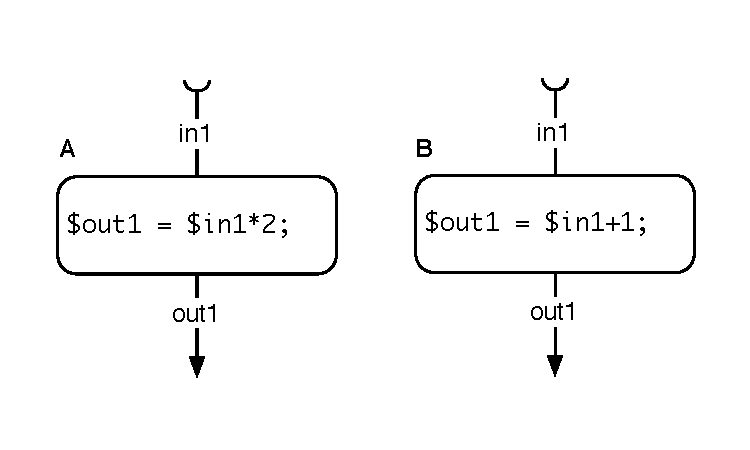
\includegraphics[width=0.75\columnwidth]{images/code-gen1}
\caption{Two basic blocks, A and B. Inputs are on top, outputs on the bottom.}
\label{fig:blocks}
\end{figure}

To accomplish block sequencing in C, Twig generates variable names such that the output(s) of the first block in the sequence are the same as the inputs(s) of the second, and the text is concatenated. See Figure~\ref{fig:codegen-seq} for an example.

\begin{figure}[ht]
\centering
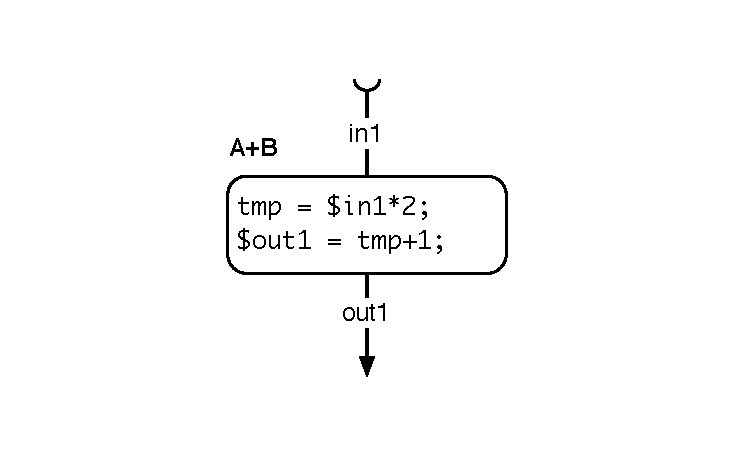
\includegraphics[width=0.75\columnwidth]{images/code-gen2}
\caption{Two blocks from Figure~\ref{fig:blocks} composed sequentially. The variable ``tmp'' is created, and renaming performed, so that the output of block A would flow to the input of block B.}
\label{fig:codegen-seq}
\end{figure}

Parallel composition for C is accomplished similarly; Twig generates independently-named variables for the inputs and outputs of the two blocks, and then concatenates the text. An example is shown in Figure~\ref{fig:codegen-par}.

\begin{figure}[ht]
\centering
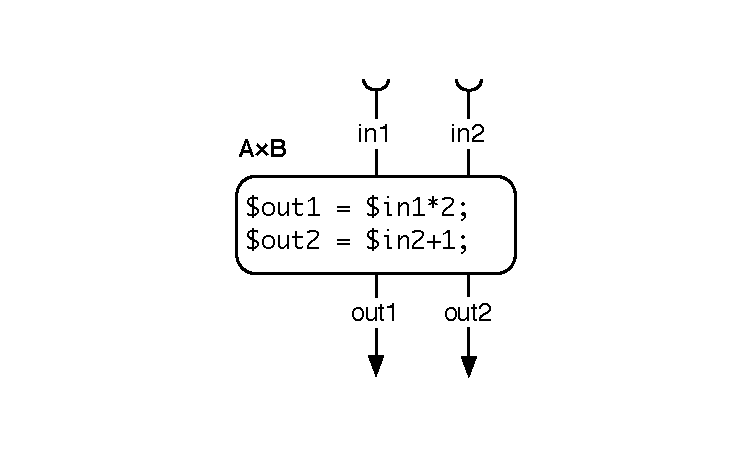
\includegraphics[width=0.75\columnwidth]{images/code-gen3}
\caption{Two blocks from Figure~\ref{fig:blocks} composed in parallel. Renaming is performed such that the composed block has two inputs and two outputs.}
\label{fig:codegen-par}
\end{figure}

Finally, to implement the special permutation and identity blocks, it suffices to perform the appropriate bookkeeping on the variable names. The identity block, $I_1$, requires no generated code at all -- the variable name on the input is simply used for the output as well. More complex permutations work similarly -- Twig will rearrage the generated variable names, but no actual code needs to be generated.

Note that this implementation does not allocate or free memory, or otherwise perform resource management as part of the permutation operations. This implies that the generated code will follow C's semantics for passing by value versus reference. The Twig user must keep these rules in mind when designing and using C typemaps.
